\documentclass{article}
\usepackage[cm]{fullpage} %very small margins (around 1.5cm)
\usepackage[utf8]{inputenc} %sets input encoding to UTF-8, needed for Polish, Japanese, etc.
\usepackage[T1]{fontenc} %needed for Polish characters
\usepackage{lmodern} %this font handles Polish characters properly

\PassOptionsToPackage{usenames,dvipsnames,svgnames}{xcolor}

%this file must be included in the preamble

\usepackage{graphicx} %use \includegraphics[scale=1.00]{file.jpg} for images
\usepackage[unicode]{hyperref}

\hypersetup{
  bookmarksopen,
  bookmarksopenlevel=1,
  pdfborder={0 0 0},
  %pdfpagelayout={SinglePage},
  %pdfstartview={FitH},
  pdfdisplaydoctitle
}

\def\logoleft#1{\gdef\logoleftpath{#1}}
\def\logoleftpath{\errmessage{Please define the logoleft}}

\def\logoleftscale#1{\gdef\logoleftscaletext{#1}}
\def\logoleftscaletext{\errmessage{Please define the logoleftscale}}

\def\logoright#1{\gdef\logorightpath{#1}}
\def\logorightpath{\errmessage{Please define the logoright}}

\def\logorightscale#1{\gdef\logorightscaletext{#1}}
\def\logorightscaletext{\errmessage{Please define the logorightscale}}

\def\title#1{\gdef\titletext{#1}\hypersetup{pdftitle={#1}}}
\def\titletext{\errmessage{Please define the title}}

\def\author#1{\gdef\authortext{#1}\hypersetup{pdfauthor={#1}}}
\def\authortext{\errmessage{Please define the author}}

\def\supervisor#1{\gdef\supervisortext{#1}}
\def\supervisortext{\errmessage{Please define the supervisor}}

\def\date#1{\gdef\datetext{#1}}
\def\datetext{\errmessage{Please define the date}}

\def\university#1{\gdef\universitytext{#1}}
\def\universitytext{\errmessage{Please define the university}}

\def\faculty#1{\gdef\facultytext{#1}}
\def\facultytext{\errmessage{Please define the faculty}}

\def\location#1{\gdef\locationtext{#1}}
\def\locationtext{\errmessage{Please define the location}}

\def\description#1{\gdef\descriptiontext{#1}}
\def\descriptiontext{\errmessage{Please define the description}}

\renewcommand{\maketitle}{
\pdfbookmark[1]{Title page}{titlepage}
\begin{titlepage}
\begin{center}
  \begin{minipage}{.15\textwidth}
    \begin{flushleft}
      \includegraphics[scale=\logoleftscaletext]{\logoleftpath}
    \end{flushleft}
  \end{minipage}
  \begin{minipage}{.66\textwidth}
    \begin{center}
      { \Large \universitytext }
    \end{center}
    
    \begin{center}
      { \Large \facultytext }
    \end{center}
  \end{minipage}
  \begin{minipage}{.15\textwidth}
    \begin{flushright}
      \includegraphics[scale=\logorightscaletext]{\logorightpath}
    \end{flushright}
  \end{minipage}
\end{center}

\vspace*{\fill}
  
\begin{center}
  \textsc{\Huge \titletext }
\end{center}
  
\begin{center}
  \textsc{ \descriptiontext }
\end{center}

\vspace*{\fill}

\hspace{.5\textwidth}
\begin{minipage}[t]{.4\textwidth}
  \begin{flushleft}
    {\large Author: \newline \authortext }
  \end{flushleft}
  
  \begin{flushleft}
    {\large Supervisor: \newline \supervisortext }
  \end{flushleft}
\end{minipage}

\vspace{50pt}

\begin{center}
  {\large\locationtext, \datetext}
\end{center}
\end{titlepage}
}


\logoleft{../../graphics/logo_pw.jpg}
\logoleftscale{0.395}
\logoright{../../graphics/logo_mini.png}
\logorightscale{0.16}
\university{Warsaw University of Technology}
\faculty{Faculty of Mathematics and~Computer~Science}
\location{Warsaw}
\supervisor{dr Lucjan Stapp} %prof. nzw. dr hab. Władysław Homenda\newline
\title{$\Phi$nite}
\description{application for building finite automaton that is equivalent to a given regular
expression \newline and for simulating machine's evaluation of a given word}
\author{Mateusz Bysiek}
\date{14 Mar 2013}

%this file must be included in the preamble

\usepackage{booktabs} %use \begin{tabular}{} with \toprule \midrule \bottomrule
\usepackage{tabulary}

\def\company#1{\gdef\companytext{#1}}
\def\companytext{\errmessage{Please define the company}}

\def\documentsubject#1{\gdef\documentsubjecttext{#1}}
\def\documentsubjecttext{\errmessage{Please define the documentsubject}}

\def\documenttopicslist#1{\gdef\documenttopicslisttext{#1}}
\def\documenttopicslisttext{\errmessage{Please define the documenttopicslist}}

\def\filename#1{\gdef\filenametext{#1}}
\def\filenametext{\errmessage{Please define the filename}}

\def\version#1{\gdef\versiontext{#1}}
\def\versiontext{\errmessage{Please define the version}}

\def\status#1{\gdef\statustext{#1}}
\def\statustext{\errmessage{Please define the status}}

\def\openingdate#1{\gdef\openingdatetext{#1}}
\def\openingdatetext{\errmessage{Please define the openingdate}}

\def\documentsummary#1{\gdef\documentsummarytext{#1}}
\def\documentsummarytext{\errmessage{Please define the documentsummary}}

% \def\#1{\gdef\text{#1}}
% \def\text{\errmessage{Please define the }}

\newcommand{\tableheader}[1]{\textbf{\large {#1}}}
\newcommand{\fieldheader}[1]{\textbf{\footnotesize {#1}}}

\newcommand{\documentmetric}{
\pdfbookmark[1]{Document metric}{docmetric}
\begin{center}
\begin{tabulary}{\textwidth}{LJLJLJ}
\toprule
\multicolumn{6}{l}{\tableheader{Document metric}} \\
\midrule
\fieldheader{Project} & \multicolumn{3}{l}{\textsc{\titletext}} 
& \fieldheader{Company} & \companytext \\
\midrule    
\fieldheader{Document name} & \multicolumn{5}{l}{\documentsubjecttext} \\
\midrule
\fieldheader{Document topics} & \multicolumn{5}{l}{\documenttopicslisttext} \\
\midrule
\fieldheader{Author} & \multicolumn{5}{l}{\authortext} \\
\midrule
\fieldheader{File} & \multicolumn{5}{l}{\filenametext} \\
\midrule
\fieldheader{Version no.} & \versiontext 
& \fieldheader{Status} & \statustext
& \fieldheader{Opening date} & \openingdatetext \\
\midrule
\fieldheader{Summary} & \multicolumn{5}{l}{\parbox{.80\textwidth}{\documentsummarytext}
} \\
\midrule
\fieldheader{Authorized by} & \multicolumn{3}{l}{\parbox{.40\textwidth}{\supervisortext}} 
& \fieldheader{Last modification date} & \datetext \\
\bottomrule
\multicolumn{6}{l}{\makebox[.96\textwidth]{}} \\
\end{tabulary}
\end{center}
}

\newcommand{\historyofchanges}[1]{
\pdfbookmark[1]{History of changes}{dochistory}
\begin{center}
\begin{tabulary}{\textwidth}{LLLJ}
\toprule
\multicolumn{4}{l}{\tableheader{History of changes}} \\
\midrule
\fieldheader{Version} & \fieldheader{Date} & \fieldheader{Author} & \fieldheader{Description} \hspace*{\fill} \\
#1
\bottomrule
\multicolumn{4}{l}{\makebox[.96\textwidth]{}} \\
\end{tabulary}
\end{center}
}

\newcommand{\change}[4]{
\midrule
{#1} & {#2} & {#3} & {#4} \\
}


\company{WUT}
\documentsubject{business analysis}
\documenttopicslist{initial analysis of the problem, requirements specification, guidelines}

\documentsummary{Author of the document analyses the problem of designing an application for solving
a well defined language\mbox{-}theory related problem, doing it from the business perspective, i.e.
giving set of requirements that such application must fulfill and providing guidelines for
developers.}

\openingdate{21 Feb 2013}
\version{0.09}
\status{pre-alpha}
\filename{bysiekm-business-analysis.pdf}

%this file must be included in the preamble

\usepackage{color}
\usepackage[usenames,dvipsnames]{xcolor}
\usepackage{lastpage} %page x of y with: \cfoot{\thepage{} of \pageref{LastPage}}
\usepackage{fancyhdr} % also needed for footers

\fancyhead{}
\fancyfoot{}
\lfoot{{ \footnotesize \textcolor{gray}{\authortext} }}
\cfoot{{ \footnotesize page \thepage{} of \pageref{LastPage} }}
\rfoot{\textsc{ \footnotesize \textcolor{gray}{\titletext, v.\versiontext} }}
\pagestyle{fancy}
\renewcommand{\headrulewidth}{0pt}
\renewcommand{\footrulewidth}{0pt}


\usepackage{amsmath}
\usepackage{amsfonts}
\usepackage{multicol} %use \begin{multicols}{#} for # columns
\usepackage{enumitem} %remove vertical space in itemize with: [noitemsep,nolistsep]
\usepackage{tikz}

\usetikzlibrary{arrows,positioning,automata}

\newcommand{\writehere}{\textbf{\textcolor{red}{Write here!}}}

\begin{document}

\maketitle

\newpage

\setcounter{page}{2}

\documentmetric

\vspace*{\fill}

\historyofchanges{
\change{0.01}{\openingdatetext}{\authortext}{creation of template for the document}
\change{0.02}{23 Feb 2013}{\authortext}{outline of the features section}
\change{0.03}{25 Feb 2013}{\authortext}{added definitions section}
\change{0.04}{25 Feb 2013}{\authortext}{added algorithm section}
\change{0.05}{27 Feb 2013}{\authortext}{added GUI mockup, moved definitions}
\change{0.06}{28 Feb 2013}{\authortext}{added use cases}
\change{0.07}{8 Mar 2013}{\authortext}{removed GUI mockup}
%\change{0.08}{8 Mar 2013}{\authortext}{removed GUI mockup}
\change{\versiontext}{10 Mar 2013}{\authortext}{added word evaluation feature}
%\change{\versiontext}{\datetext}{\authortext}{added use cases}
}

\newpage

\tableofcontents

\newpage


\section*{Abstract}

This document describes a business analysis (problem analysis and requirements specification) of a
planned application called \titletext. This application is aimed at introducing the user to the
world of regular expressions\textsuperscript{\cite{wiki_rl}} and finite-state
machines\textsuperscript{\cite{wiki_fsm}} (i.e. the theoretical constructs that let us evaluate
regular expressions). The application will consist of GUI (graphical user interface) coupled with a
regular expression evaluation engine. Together these two components will enable the user to enter an
expression by hand (or, alternatively, load it from a list of prepared examples) and then
semi-automatically construct a finite-state machine that is equivalent to this expression.
In other words, given regular expression expands into the same set of words that a resulting
finite-state machine accepts.

Furthermore, the user will be able to simulate how the built finite-state machine works for a given
input word.

\section{Feature overview}
In this section, reader is presented with the features that must be implemented, unless a given
feature is explicitly labeled as: optional, not mandatory, etc. The application will fulfill the
requirements if it implements all of the given features, unless those features are impossible to
implement while meeting the application environment constraints.

\subsection{Input methods}
Some definitions are vital in proper understanding of the calculation methods described below, and
in proper understanding of the requirements.

\subsubsection*{Definition}
\begin{itemize}

  \item \textit{input data} is a sequence of characters, which can be converted to a valid regular
  expression without ambiguity, and without user interaction.

\end{itemize}

Those characters must be writable with regular plain text editor. Moreover, the input data should,
unless it is impossible in certain cases, be visually similar to a regular expression that is
written without plain text editor. Using \LaTeX{} math mode syntax is preferred, but not
mandatory.

Ex. ``\verb|ab^*|'' under a set of not ambiguous rules may represent $ab^*$, and on the other hand,
there is no set of unambiguous rules to convert \verb|(ab)*(| to a regular expression. The latter
may represent $(ab)\ast($ i.e. a word in which parentheses and other special characters denote
letters (preventing the user from using parentheses - which is unacceptable), or maybe $(ab)^*($
where the last parenthesis serves as a letter, and the two first are parentheses. The opening
parenthesis may have different meaning depending on context - it is also unacceptable.

\subsubsection*{Requirements}

The user shall be able to enter the regular expression using at least
% three
two methods described below:
\begin{itemize}

  \item \textit{direct input} - user writes the expression into a single- or multi-line plain text
  field in the GUI.

  %\item load from plain text file

  \item \textit{example selection} -  user selects expression from a list of predefined expressions.
  There should be at least 10 example expressions, and they (globally) have to show usage of:
  \begin{itemize}[noitemsep,nolistsep]

    \item \textit{empty word}, ex. $\epsilon$

    \item \textit{concatenation}, ex. $ab$ is a concatenation of $a$ and $b$

    \item \textit{union}, ex. $a+b$, which generates $a$ and $b$, and is equivalent to $b+a$

    \item \textit{Kleene star}\textsuperscript{\cite{wiki_kleenestar}}, ex. $a^*$, which generates a
    set of concatenations of $a$ with itself $n \in \mathbb{N}\cup\{0\}$ times, and is equivalent to
    $\epsilon+a^+$

    \item \textit{Kleene plus}\textsuperscript{\cite{wiki_kleenestar}}, ex. $a^+$, which generates a
    set of concatenations of $a$ with itself $n \in \mathbb{N}\backslash\{0\}$ times, and is
    equivalent to $aa^*$

    \item \textit{precedence of operators} (i.e. the use of parentheses and/or their absence), ex.
    $ab^+$, is equivalent to $abb^*$, but $(ab)^+$ is equiv. to $ab(ab)^*$

  \end{itemize}
  
  The selected example expression is loaded into the text field mentioned in the first input method,
  overwriting any previous input.

\end{itemize}

\subsection{Input editing methods}
The user will be able to edit the expression regardless of what the input method was, before he/she
proceeds with calculations. Editing the input is to be done via a plain text field in the GUI.

\subsection{Calculation methods}
\label{sec:calcmethods}

\subsubsection*{Definitions}
\begin{itemize}%[noitemsep,nolistsep]

  \item \textit{one step of computation} is a smallest step that can be taken from the algorithm
  used to complete calculations (in this case it is to find finite-state machine equivalent to the
  given regular expression).

  \item \textit{visualisation of current status of computation} consists of two tables that
  represent (respectively) the labeling and derivation process undertaken by the program (see
  section~\ref{sec:solutionprocess} for details regarding labeling and derivation process).

\end{itemize}

The first tables shows all currently labeled and not labeled symbols, therefore has to have at least
two columns: regular expression, and label. When second field is empty then the expression is not
labeled. If the algorithm is currently in labeling phase, the currently evaluated non-labeled
expression is highlighted.

The second table has at list three columns: initial expression, subtracted symbol, resulting
expression. If the algorithm is currently in derivation phase, the currently derived expression is
highlighted.

Highlighting means that either 1) the background color of a cell in which a highlighted content
resides is changed to the font color, and the font color is changed to the background color or 2)
background color of a cell has color changed from white to gray (between \verb|#c0c0c0| and
\verb|#808080|, inclusive).

\subsubsection*{Requirements}
The user will be able to convert the entered expression to an equivalent finite-state machine using
two methods:
\begin{itemize}

  \item \textit{immediate result method}: will proceed with calculations up to the moment when user
  interaction is necessary, and will show visualisation of current status of computation only in
  such situation. After such pause, when the user decides to end interaction, he/she will click a
  button that will cause the computation to continue.
  
  This method completes when there are no intermediate steps that need user interaction and the
  final result is presented in the GUI.

  \item \textit{step-by-step method}: will perform one step of computation and present visualisation
  of current status of computation to the user. At that point the user can choose whether he/she
  would like to:
  
  \begin{itemize}

    \item proceed with the next step of computation

    \item abort computation, effectively reverting to the beginning

    \item proceed with the computation using \textit{immediate result method}, starting from the
    current position

  \end{itemize}
  
  This method completes when there are no more steps needed to obtain the final result.
  
  In this method, user still might be obliged to perform some actions in between steps, as it is
  possible in case of \textit{immediate result method}. In such cases, the 3 options for typical
  continuation shall be disabled, and only after the user indicates that the intermediate
  interaction is finished, they are enabled again and the user may choose further course of action.

\end{itemize}

\subsection{Output analysis methods}

\subsubsection*{Definition}
\begin{itemize}[noitemsep,nolistsep]

  \item \textit{final result} is a two-dimensional directed graph with labeled edges. It is a
  graphical representation of a finite state machine constructed.

\end{itemize}

\subsubsection*{Requirements}
Final result has to conform with several constraints, most of which follow directly from the
convention regarding drawing finite-state machines:
\begin{itemize}

  \item all vertices, letters and edges on the graph have to be black and the background has to be
  white

  \item the vertices have to be black circles, and those representing accepting states have to have
  another black circle inside

  \item the initial state has to have index $0$ ex. it can be $q_0$, $s_0$, $r_0$, \ldots

  \item the edges leading to the rejecting state should be omitted for better readability, and the
  rejecting state is not to be drawn at all

  \item the drawing has to be readable, i.e. font size used has to be at least 10 points.

  \item if the drawing is too big to fit in applicatin window or on user's screen, the output is not
  zoomed out but rather a method must be implemented so that the user can scroll around the drawing
  to be able to see everything piece by piece.

\end{itemize}

\subsection{Simulation methods}

\subsubsection*{Definition}
\begin{itemize}[noitemsep,nolistsep]

  \item \textit{finite-state machine simulation} is a process of evaluation of a sequence
  of letters given by the user using a finite-state machine.

\end{itemize}

\subsubsection*{Requirements}
The finite-state machine simulation must conform with the following requirements:
\begin{itemize}

  \item the simulation should be done step-by-step, much like in the case of machine construction
  process, but the difference is that the feature of immediate solution may be ommited
  (see requirements part in section~\ref{sec:calcmethods} for details regarding solution methods)
  
  \item the evaluation is represented graphically, i.e. the requirements regarding graphical
  representation of the output apply to the finite-state machine simulation

  \item in each step the node that represents the current state of the machine is highlighted (see
  the end of definitions in section~\ref{sec:calcmethods})
  
  \item if a rejecting state is entered than no node is highlighted anymore and the message window
  is displayed that informs the user that the word was rejected by the machine
  
  \item if there are no more letters for evaluation and current state is not an accepting state, the
  message window (analogous to the one in the previous point) is displayed
  
  \item if an accepting state is entered and there are no more letters remaining for evaluation, the
  message window is displayed that informs the user that the word was accepted by the machine

\end{itemize}

\section{Building finite-state machine: workflow with example}
The computation process used by the application shall follow the following outline. Solutions to two
sub-problems:
\begin{itemize}

  \item determining if some regular expression is equivalent to some other expression

  \item determining whether some regular expression can generate an empty word

\end{itemize}

\ldots do not have to be implemented, and can be left out for the user interaction. However, when
algorithm requires user interaction, it has to stop and show to the user all the needed information
so that he/she can really perform a task using only data provided by the application. The
development team is free to choose at which steps the the algorithm will be interactive.

\subsection{Input}
Input is in every case a valid regular expression. Further steps cannot be performed until the given
input satisfies validity criterion.

Example input:
\begin{gather*}
a^+c^+ + ab^+c
\end{gather*}

This expression represents a following set of words:
\begin{gather*}
L = \left\{ ac, aac, aaac, aaaac, \ldots \right\} %\cup \\
\cup \left\{ acc, aacc, aaacc, aaaacc, \ldots \right\} %\cup \\
\cup \left\{ accc, aaccc, aaaccc, aaaaccc, \ldots \right\} \cup \\
\cup \left\{ acccc, aacccc, aaacccc, aaaacccc, \ldots \right\} %\cup \\
\cup \ldots %\cup \\
\cup \left\{ abc, abbc, abbbc, abbbbc, \ldots \right\}
\end{gather*}

\subsection{Task}
Task is the same for every input: ``construct a finite-state machine equivalent to a given regular
expression''.

\subsection{Solution process}
\label{sec:solutionprocess}
In this part FSM is used as an acronym for finite-state machine.

\subsubsection{Step 0}
\label{sec:step0}

\subsubsection*{Labeling, step $0_L$}
At first we label our input as an initial state of the FSM:
\begin{gather*}
a^+c^+ + ab^+c = q_0
\end{gather*}

\subsubsection*{Derivation, step $0_D$}
Then, we try to derive all states of FSM that can be reached from our initial state in one
transition.

$e / x$ means that we try to construct from expression $e$ a new  expression without initial symbol
$x$, provided that such expression exists. If it does not, the result is the empty set:
\begin{gather*}
q_0 / a = a^*c^+ + b^+c \\
q_0 / b = \emptyset \\
q_0 / c = \emptyset
\end{gather*}

\subsubsection{Steps 1 to N+1}

\paragraph{Labeling, step $1_L$}
In each of these steps we at first label all results from the last step as new states of the FSM,
unless the equivalent expressions were previously encountered and are already labeled.
\begin{gather*}
a^*c^+ + b^+c = q_1
\end{gather*}

\paragraph{Derivation, step $1_D$}
Then we take the first unresolved state from the list of labeled states and we perform the same
operation as in Step $0_D$ (described in point~\ref{sec:step0}):
\begin{gather*}
q_1 / a = a^*c^+ \; , \;
q_1 / b = b^*c \; , \;
q_1 / c = c^*
\end{gather*}

\begin{multicols}{2}

\paragraph{Labeling, step $2_L$} $a^*c^+ = q_2$, $b^*c = q_3$, $c^* = q_4$

\paragraph{Derivation, step $2_D$} $q_2 / a = a^*c^+$, $q_2 / b = \emptyset$, $q_2 / c = c^*$

\paragraph{Step $3_L$} $a^*c^+$ and $c^*$ are already labeled

\paragraph{Step $3_D$} $q_3 / a = \emptyset$, $q_3 / b = b^*c$, $q_3 / c = \epsilon$

\paragraph{Step $4_L$} $b^*c$ is already labeled, $\epsilon = q_5$

\paragraph{Step $4_D$} $q_4 / a = \emptyset$, $q_4 / b = \emptyset$, $q_4 / c = c^*$

\paragraph{Step $5_L$} $c^*$ is already labeled

\paragraph{Step $5_D$} $q_5 / a = \emptyset$, $q_5 / b = \emptyset$, $q_5 / c = \emptyset$

\paragraph{Step $6_L$} There are no states to label in this step. There may be some unresolved
states, therefore we cannot end computation at this moment.

\paragraph{Step $6_D$} There are no more unresolved states, the algorithm moves to the next stage.

\end{multicols}

\subsubsection{Step N+2}
After derivation from all states (total number of states of the resulting FSM is $N+1$), each state
is evaluated and it is determined if an expression equivalent to the state can generate an empty
word ($\epsilon$). If yes, such state is added to the set of accepting states. Initial state can
also be an accepting state. There can be only one initial state, but multiple accepting states are
possible.

In our example $c^* = q_4$ and $\epsilon = q_5$, therefore $Q_A = \{ q_4, q_5 \}$
 
There is a special case, an empty state, which is the rejecting state. There is only one rejecting
state.

\subsection{Final result}
Final result is a transformation of a record of computation process into a graph that represents it.
\begin{gather*}
\begin{cases}
q_0 / a = q_1 \\
q_0 / b = \emptyset \\
q_0 / c = \emptyset
\end{cases}
\mbox{ is transformed into }
\begin{cases}
q_0 \overset{a}{\rightarrow} q_1 \\
q_0 \overset{b}{\rightarrow} \emptyset \\
q_0 \overset{c}{\rightarrow} \emptyset
\end{cases}
\end{gather*}

Analogously, every other derivation that happened in the steps $1_D \ldots N_D$ is transformed in
the same way. After all derivations are transformed a graph is drawn in the GUI.

Rules regarding the graph are as follows:
\begin{itemize}

  \item states $q_0, q_1, \ldots, q_n$ become the set of vertices

  \item transition $q_i \overset{x}{\rightarrow} q_j$ becomes a labeled and directed edge from vertex $q_i$ to
  vertex $q_j$, with label ``$x$''

\end{itemize}

This concludes a complete computation process.

\begin{figure}[ht!]
  \centering
  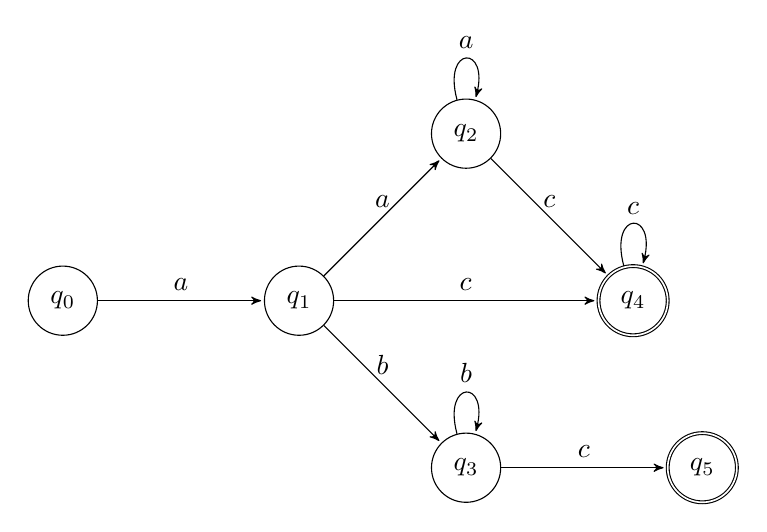
\begin{tikzpicture}
    [>=stealth',shorten >=1pt,node distance=3cm,on grid,initial/.style={}]

    \node[initial,state] (q0) {$q_0$};
    \node[state] (q1) [right =of q0] {$q_1$};
    \node[state] (q2) [above right =of q1] {$q_2$};
    \node[state] (q3) [below right =of q1] {$q_3$};
    \node[state,accepting] (q4) [below right =of q2] {$q_4$};
    \node[state,accepting] (q5) [right =of q3] {$q_5$};

    \path
    (q0) edge [->,above] node {$a$} (q1)
    (q1) edge [->,above] node {$a$} (q2)
    (q1) edge [->,above] node {$b$} (q3)
    (q1) edge [->,above] node {$c$} (q4)
    (q2) edge [loop above] node {$a$} (q2)
    (q2) edge [->,above] node {$c$} (q4)
    (q3) edge[loop above] node {$b$} (q3)
    (q3) edge [->,above] node {$c$} (q5)
    (q4) edge [loop above] node {$c$} (q4)
    ;

  \end{tikzpicture}
  \caption{graphical representation of the final answer for the example problem}
\end{figure}

%\section{Word evaluation: workflow with example}

%\subsection{Input}

%\subsection{Solution process}

%\subsection{Final solution}

\section{Use cases}

Below is the diagram that puts the given requirements into a UML diagram. Division of the
application into two parts as pictured is a recommendation. Input/output handler is meant to
comprise the features related to getting the regular expression from the user, validating it, and
also displaying the final result. Computing process is meant to handle conversion related
calculations, without direct input from the user, but is able to receive suggestions regarding
computation form him/her.

\begin{figure}[ht!]
  \centering
  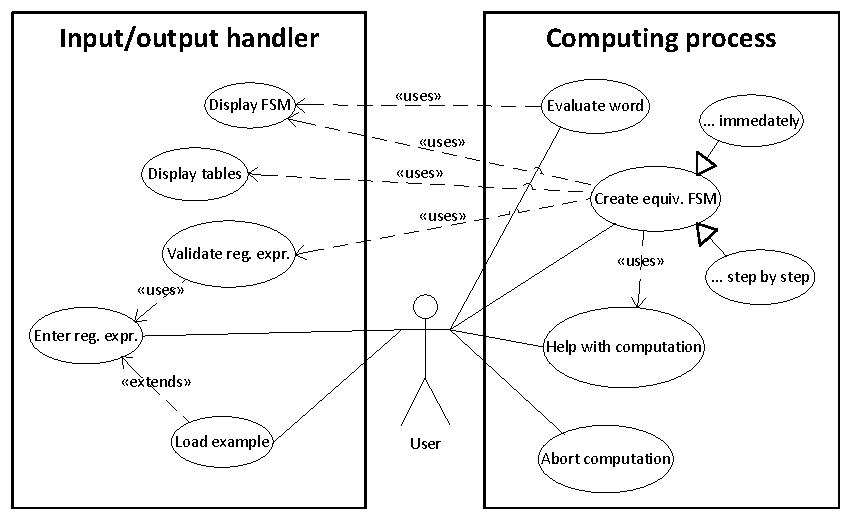
\includegraphics[width=\textwidth]{../../use_case/use_cases.pdf}
  \caption{UML use case diagram for \titletext{} user}
\end{figure}

\section{Exception handling}
The theoretical background behind the concept of regular languages is very well established. This
application will therefore implement no experimental features, and undefined behaviour is strictly
forbidden.

The exception from this rule is a situation in which user input is needed during computation (there
are two cases), and the amount of work the user has to do in order to submit his/her help is lowered
due to some supporting experimental features, that may not always work, but sometimes help the user.
Such solutions will be considered an advantage, but are not a must.

In order to ensure that the computation will proceed as expected, application will perform
validation of input. Such validation does not have to be performed on per-character-written basis.
It is required for the program to validate input when user attempts to commence computation. At this
point, if the validation fails, either:

\begin{itemize}

  \item a message window is presented with information about this fact,

  \item or text box with the input data is highlighted by changing its border to red line that has
  width between 2 and 4 pixels; and text informing the user about the error is added to the status
  bar.

\end{itemize}

Program will prohibit user from changing input data after the computation has started. Editing
capabilities will be restored after the computation has finished, or after the user aborts current
computation before it has concluded and the final solution is presented.

\newpage

\begin{thebibliography}{9}

\bibitem{wiki_rl}
  Wikipedia contributors,
  \emph{Regular language},
  2013
  \url{https://en.wikipedia.org/wiki/Regular_language}, accessed 25 Feb 2013.

\bibitem{wiki_fsm}
  Wikipedia contributors,
  \emph{Finite-state machine},
  2013
  \url{https://en.wikipedia.org/wiki/Finite-state_machine}, accessed 23 Feb 2013.

\bibitem{wiki_kleenestar}
  Wikipedia contributors,
  \emph{Kleene star},
  2013
  \url{https://en.wikipedia.org/wiki/Kleene_star}, accessed 25 Feb 2013.

\end{thebibliography}

\end{document}
